\label{sec:def}

To establish a rigorous foundation for World Action Models (WAMs), we define the embodied intelligence task through a probabilistic lens. We consider an embodied agent interacting with an environment. 
At each timestep, the agent receives an observation 
$o \in O$ (encompassing visual inputs, proprioceptive 
signals, and any other sensory modalities), a language instruction 
$l \in L$, and produces actions $a \in A$. 
We use $o'$ to denote the observation at the subsequent timestep.

\subsection{Foundational Paradigms}

\begin{figure}
    \centering
    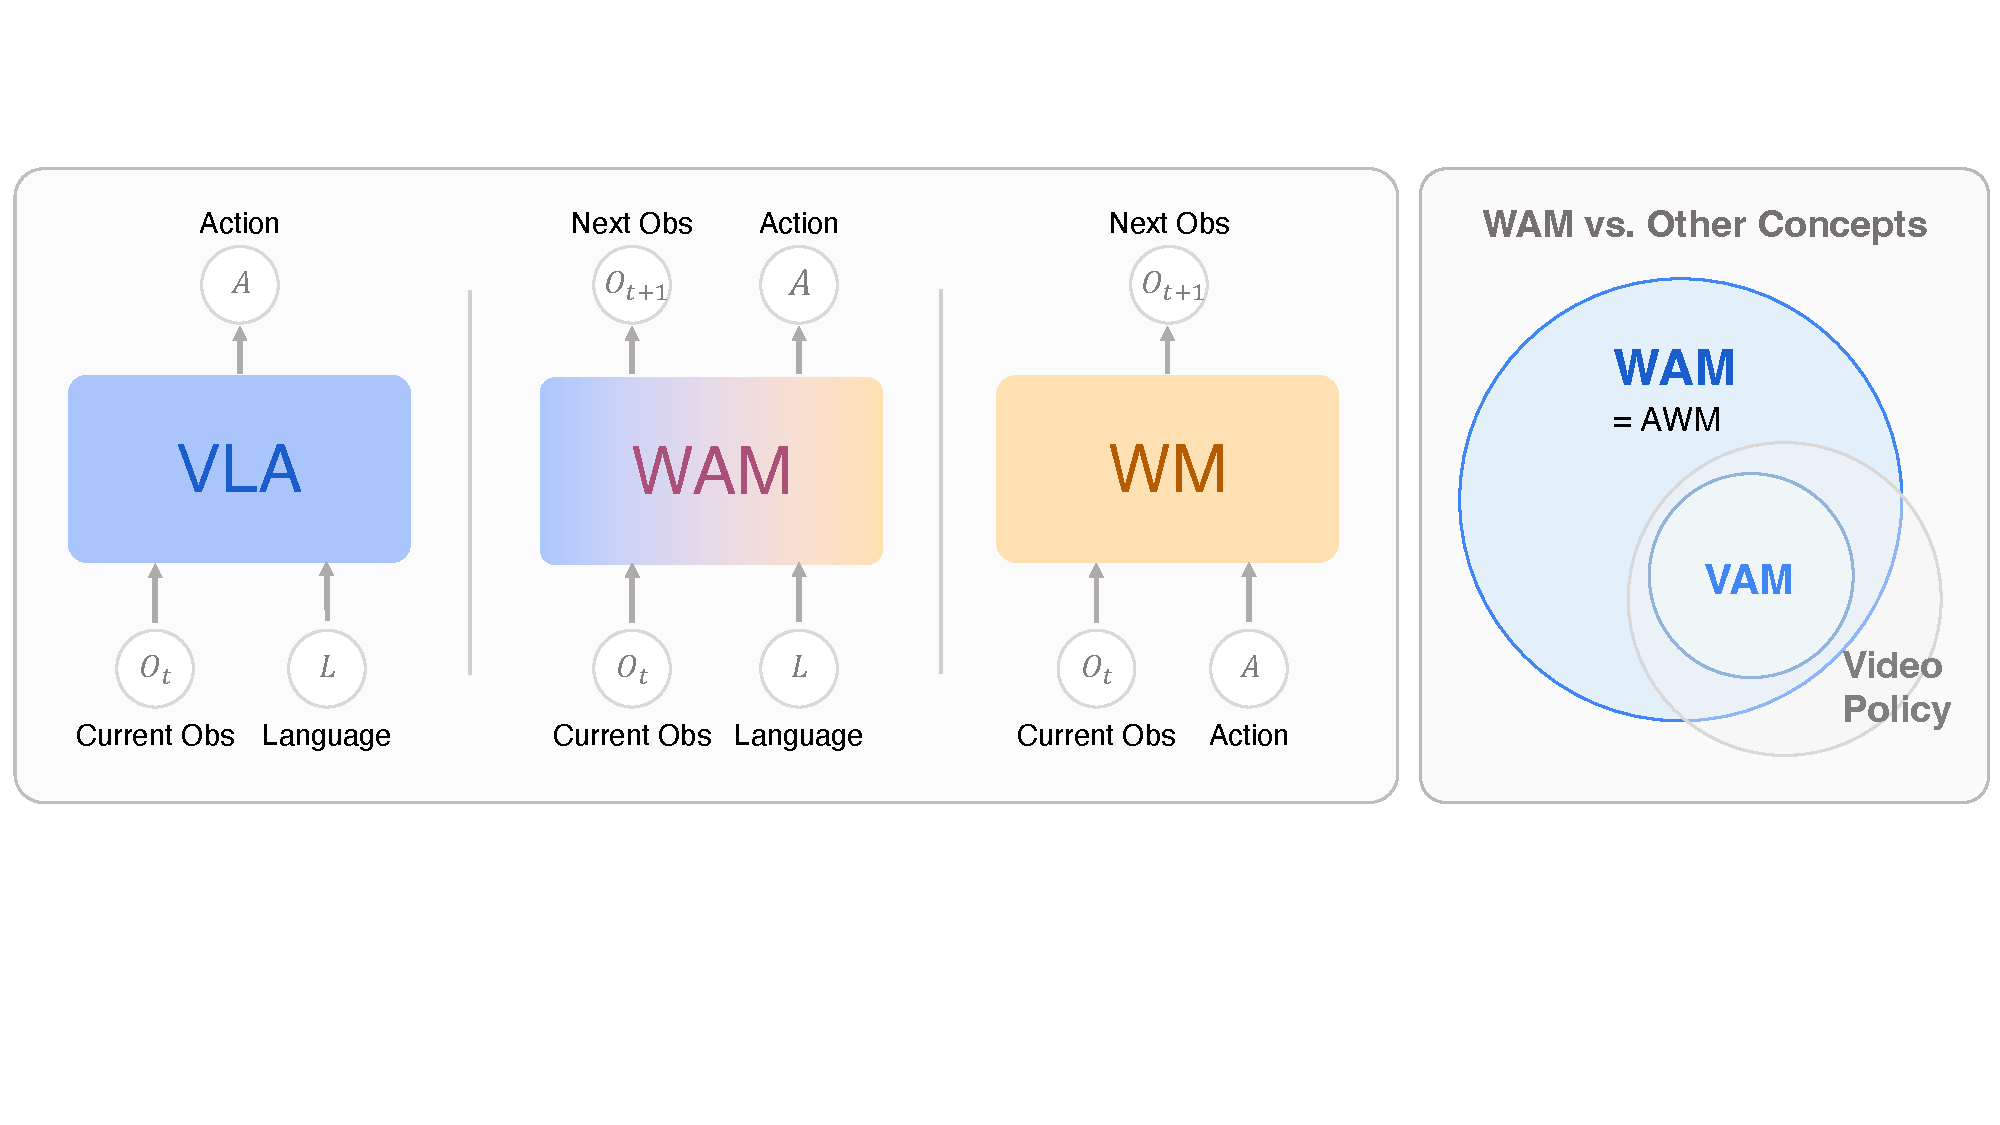
\includegraphics[width=1\linewidth]{pic/def.pdf}
    \caption{Conceptual definition and comparison of World Action Models (WAMs). The left panel contrasts the input-output formulations of Vision-Language-Action (VLA) models, WAMs, and standard World Models (WMs), highlighting WAM's capability to jointly predict actions and future observations. The right panel illustrates the conceptual scope of WAMs relative to other paradigms such as Video Action Models (VAMs) and Video Policies.}
    \label{fig:definition}
\end{figure}

\textbf{Vision-Language-Action (VLA)} models are a class of embodied foundation models that frame robot control as a multimodal sequence modeling task. In this paradigm, the agent processes current observation $o$ and linguistic instructions $l$ to generate a sequence of action tokens $a$. The VLA architecture typically leverages the pre-trained semantic latent spaces of Large Language Models (LLMs) or Vision-Language Models (VLMs) to map perceptual inputs directly to the action space. Formally, the VLA objective is defined by the conditional probability of actions given the multimodal context:

% VLA
$$ \mathcal{L}_{\text{VLA}} = \mathbb{E}_{(o, l, a) \sim \mathcal{D}} \left[-\log p(a \mid o, l)\right] $$



\textbf{World Models (WM)} 
are defined as predictive transition functions that internalize the causal dynamics of the physical environment. The functional role of a WM is to model the forward-dynamics of the world—simulating the evolution of environmental observed states $o'$ conditioned on a preceding state $o$ and a sequence of hypothetical interventions $a$. This is typically expressed as:

% WM
$$\mathcal{L}_{\text{WM}} = \mathbb{E}_{(o, a, o') \sim \mathcal{D}} 
\left[-\log p(o' \mid o, a)\right]$$


Within this framework, the model acts as a probabilistic propagator of states, providing a representation of how the environment changes in response to specific actions.


\textbf{World Action Models (WAMs)} are a class of embodied foundation models that unify environmental dynamics modeling (world modeling) with motor control (action generation). Unlike standard Vision-Language-Action (VLA) models that learn direct observation-to-action mappings, WAMs predict the future evolution of the physical environment. Formally, a WAM must fulfill two core criteria: 

\begin{enumerate}
    \item \textbf{Forward Predictive Modeling:}
    The model must forecast the physical evolution of the environment by generating or utilizing a quantifiable representation of future states $o'$. This modeling can manifest as explicit visual predictions (e.g., pixel-level video frames, dense optical flow) or implicit physical representations (e.g., physics-grounded latent spaces).
    
    \item \textbf{Coupled Action Generation:} The model must deduce its motor commands $a$ by strictly aligning them with the anticipated future states $o'$. This coupling can manifest as a joint probabilistic output or as policy conditioning within a cascaded or unified latent architecture.
\end{enumerate}

Formally, a WAM seeks to characterize the joint or conditional distribution of future states and actions within a unified framework:

% WAM
$$\mathcal{L}_{\text{WAM}} = \mathbb{E}_{(o, l, o', a) \sim \mathcal{D}} \left[-\log p(o', a \mid o, l)\right].$$


By moving beyond observation-to-action mapping towards joint state-action prediction, WAMs leverage rich spatiotemporal priors to achieve deeper physical understanding and stronger zero-shot generalization.


\subsection{Disambiguation: WAM vs. Related Concepts}

To ensure conceptual clarity, we distinguish World Action Models (WAMs) from several related concepts in the generative robotics literature.

\begin{enumerate}
    \item \textbf{Video Action Models (VAMs):} 
    VAMs often refer to the models that integrate video prediction with action generation, typically aligning action with synthesized visual futures.
    We define WAMs as a broader, modality-independent superset of predictive agents. While VAMs are specifically optimized to align actions with video frame synthesis, the WAM paradigm posits that video is merely one possible proxy for modeling the world. WAMs encompass models that utilize other predictive targets—such as single-image state transitions, dense point clouds, or multi-sensory modalities like tactile and force feedback. The term ``World'' emphasizes the model's internalization of underlying physical laws and causal dynamics, rather than a commitment to the pixel-level video format.

    \item \textbf{Video Policies:} Video policies often refer to models defined by their structural heritage—using generative video architectures (e.g., Diffusion Transformers) as a backbone to extract strong spatiotemporal representations. This distinction with WAM is rooted in two dimensions: structural heritage and predictive commitment. First, similar to the WAM/VAM distinction, \textit{Video Policies} are conceptually tied to video-generation backbones (e.g., Video Diffusion Transformers). In contrast, WAMs are backbone-agnostic and can be instantiated via any architecture capable of state synthesis across diverse modalities. Second, a model can be categorized as a video policy if it merely inherits the pre-trained spatiotemporal representations of a video model to map observations directly to actions ($p\left( a | o \right)$). A WAM, however, requires an active predictive commitment; it must be supervised by a world-modeling objective where the synthesis of the next state $o'$ is an explicit component of the model's reasoning and output, rather than just an implicit feature within the backbone. 
    
    
    \item \textbf{Action World Models (AWM):} 
    Action World Model (AWM) is employed in early literature to describe models that integrate world modeling with action generation ($p(o', a \mid o, l)$). 
    While functionally similar, the choice of WAM over AWM reflects a strategic shift in the hierarchy of embodied intelligence. In the ``AWM'' phrasing, the noun is ``World Model'', which characterizes the system as an augmented simulator. World Action Model repositions the system as a primary category of Agent, where ``World'' (predictive physics) and ``Action'' (motor control) are co-equal components. This nomenclature establishes WAM as the direct conceptual successor to the Vision-Language-Action lineage, emphasizing its identity as a complete foundation model for robotics.
\end{enumerate}

